%!TEX encoding = UTF-8 Unicode
% ================================================================================
\documentclass[
    fontsize=12pt,
    headings=small,
    parskip=half,           % Ersetzt manuelles Setzen von parskip/parindent.
    bibliography=totoc,
    numbers=noenddot,       % Entfernt den letzten Punkt der Kapitelnummern.
    open=any,               % Kapitel kann auf jeder Seite beginnen.
%   final                   % Entfernt alle todonotes und den Entwurfstempel.
    ]{scrreprt}
% ===================================Praeambel==================================
\include{stylesvs}
%\addbibresource{literaturliste}
% ===================================Dokument===================================

\title{Entwicklung eines Visualisierungswerkzeuges zur Demons-
tration datenschutzfreundlicher Dokumentspeicherdienste}
\author{David Kirchhausen Monteiro}
\nocite{*}
\begin{document}
\begin{titlepage}% {{{
\includegraphics[width=6.8cm]{../pic/up-uhh-logo-u-2010-u-farbe-u-rgb.pdf}
\begin{center}\Large
	% Universität Hamburg \par
	% Fachbereich Informatik
	\vfill
	Bachelorarbeit
	\vfill
	\makeatletter
	{\Large\textsf{\textbf{\@title}}\par}
	\makeatother
	\vfill
	vorgelegt von
	\par\bigskip
	\makeatletter
	{\@author} \par
	\makeatother
	geb. am 24. Januar 1994 in Hildesheim \par
	Matrikelnummer 6530927 \par
	Studiengang Software-System-Entwicklung
	\vfill
	\makeatletter
	eingereicht am {\@date}
	\makeatother
	\vfill
	Betreuer: Maximilian Blochberger, M. Sc. \par
	Erstgutachter: Prof. Dr.-Ing. Hannes Federrath \par
	Zweitgutachter: Tilmann Stehle, M. Sc.
\end{center}
\ifoptionfinal{}{}
\end{titlepage}% }}}

\chapter*{Aufgabenstellung}
Im  Zuge  dieser  Bachelorarbeit  soll  ein  einfacher  Dokumentenspeicher  entwickelt  werden,
welcher möglichst viele Nutzerdaten erfasst und speichert. Die erfassten Daten sollen anschaulich
grafisch dargestellt werden können. Weiter sollen verschiedene Szenarien entwickelt werden,
welche aufzeigen wie eine mögliche Benutzung des Services mit und ohne der Verwendung
von datenschutzfreundlichen Methoden zum Anonymisieren von Daten aussieht. Anhand der
Szenarien soll eine grafische Auswertung Unterschiede zwischen anonymisierten Daten und
nicht anonymisierten Daten visuell sichtbar machen und die Unterschiede somit leicht zugänglich
sein.

\chapter*{Eidesstattliche Versicherung} % war: Selbständigkeitserklärung
\vspace{1cm}

Hiermit versichere ich an Eides statt, dass ich die vorliegende Arbeit selbstständig verfasst und keine anderen als die angegebenen Hilfsmittel – insbesondere keine im Quellenverzeichnis nicht benannten Internet-Quellen – benutzt habe. Alle Stellen, die wörtlich oder sinngemäß aus Veröffentlichungen entnommen wurden, sind als solche kenntlich gemacht. Ich versichere weiterhin, dass ich die Arbeit vorher nicht in einem anderen Prüfungsverfahren eingereicht habe und die eingereichte schriftliche Fassung der auf dem elektronischen Speichermedium entspricht.

\makeatletter
Hamburg, den {\@date}
\makeatother

\vspace{2cm}
\rule{6cm}{0.25pt}\\
\makeatletter
{\@author} \par
\makeatother

\chapter*{Abstract}
Um ein mögliches Missbrauchspotential und die generelle Informationsgewinnung aus gesammelten Verkehrs- und Metadaten durch Servicebetreiber deutlich zu machen, wird im Rahmen dieser Arbeit ein einfacher Dokumentenspeicher konzipiert und implementiert.
Der Dokumentenspeicher sammelt Verkehrs- und Metadaten und besitzt ein Visualisierungstool um diese gesammelten Daten anschaulich grafisch darzustellen.
Weiter werden zwei Szenarien definiert und umgesetzt, welche die Benutzung des Dokumentenspeichers exemplarisch aufzeigen und die Visualisierungsmöglichkeiten anhand der Beispieldaten der Szenarien vorführt.
Anhand der verschiedenen Visualisierungen wird der potentielle Informationsverlust für einen Servicebetreiber, der durch die Nutzung verschiedener datenschutzfreundlicher Methoden zur Anonymisierung von Daten entsteht, sichtbar gemacht. 

\tableofcontents
\listoffigures
\addcontentsline{toc}{chapter}{Abbildungsverzeichnis}

\chapter{Einleitung} \label{Kap:Einleitung}

Dokumentenspeicherdienste sind nützliche Alltagsgegenstände, welche für private sowie kommerzielle Nutzer meist unverzichtbar sind. 
Sie bieten nicht nur den Speicherplatz für wichtige Dateien der Nutzer, sondern bieten auch Sicherheit für die Dateien und machen sie global jederzeit verfügbar. 
Durch die große Datensammlung dieser Dienstleister machen sie sich nicht nur selbst zu lukrativen Zielen von gezielten Angriffen.
Dies zeigen mehrere Fälle, in denen z.~B. von Yahoo Daten gestohlen wurden und das Ausmaß der gestohlenen Nutzerdaten \cite{Yaho17}. 
Auch die Dienstleister selber können die Daten über die Nutzer sammeln, auswerten und weiter verwenden, z.~B. die Dateigröße oder den Autor der Datei aus den Metadaten oder die IP-Adresse oder die HTTP (Hypertext Transfer Protocol) Header Felder \cite{HTTP} aus den Verkehrsdaten.
Vor allem private Nutzer sind meist gar nicht über die Risiken und das Missbrauchspotenzial aufgeklärt, welche die Verwendung solcher Dienstleistungen mit sich bringen können. 
Methoden zur Verschlüsselung oder das Anonymisieren von Daten sind Benutzern meist nicht bekannt, werden von den Dienstanbietern nicht angeboten oder sind schwer umzusetzen, da es einen meist erheblichen Aufwand für die Benutzer bedeutet und Kompetenzen erfordert, welche diese Benutzer oft nicht besitzen. 
Zudem ist Benutzern oft nicht klar, inwiefern sie Informationen über sich selbst durch die Nutzung eines Services preisgeben.
Um genau die Risiken und Missbrauchspotenziale aufzuzeigen wird im Zuge dieser Arbeit ein Dokumentenspeicherdienst entwickelt, welcher Verkehrs- und Metadaten der Nutzer sammelt und diese in einer visuellen Darstellung zusammenfasst. 
Zur Implementation des Dokumentenspeichers wird dabei das Microsoft ASP.NET Core Framework verwendet. 
Das Framework wird benutzt, um die Webbenutzeroberfläche sowie die Web API (Application programming interface) des Dokumentenspeichers zu realisieren. 
Dazu wird das Data-Driven Documents Framework (d3.js\footnote{\url{https://d3js.org/}}), zur Visualisierung der Daten verwendet. 
Der Dokumentenspeicher soll vor allem den Unterschied zwischen der Verwendung von Methoden zum Anonymisieren von Daten und ungeschützten Daten visualisieren.
Dazu verwaltet der Dokumentenspeicher zwei verschiedene Datensätze, wobei eine Datenmenge ohne und eine Datenmenge mit der Verwendung von Methoden zum Anonymisieren von Daten erzeugt wird. 
Der entstehende Unterschied der gesammelten Daten durch die verschiedenen Methoden führt dann zu einer Veränderung in der Visualisierung, was den Effekt und Nutzen der Methoden deutlich sichtbar macht. 
 
\chapter{Related Work}
Die Ergebnisse und Erkenntnisse mehrerer Arbeiten wurden in dieser Arbeit verwendet, um die Aufgabenstellung zu bearbeiten.
Dies ergab sich aus der Nähe ihrer Themen zur Aufgabenstellung und dem erarbeiteten Lösungsansatz.
Diese werden nun kurz vorgestellt.

In den Ausarbeitungen von \textcite{Ecke10} und \textcite{Boda} werden Methoden zum Erzeugen eines Fingerprints (Fingerabdruck) anhand gesammelter Daten eines Benutzers erarbeitet. 
Dieser Fingerprint soll verwendet werden, um einen Benutzer wiedererkennen zu können.
In den Arbeiten \cite{Ecke10} und \cite{Boda} wird dabei eine ähnliche Methodik zum Erzeugen des Fingerprints vorgestellt.
\textcite{Ecke10} und \textcite{Boda} verwenden beide HTTP Header und Javascript, zum Ermitteln von Informationen über einen Benutzer.

\textcite{Ecke10} betrachtet dabei die HTTP Felder \textit{User-Agent} und \textit{Accept} sowie Informationen zu Cookies (enabled/disabled).
Zusätzlich wird mittels Javascript Funktionalitäten die Bildschirmgröße, Zeitzone, Informationen zu Browserplugins und Systemfonts ermittelt und ein Test auf Supercookies durchgeführt. \cite[p. 4-5]{Ecke10}

\textcite{Boda} betrachtet ebenfalls das HTTP Headerfeld \textit{User-Agent} und sammelt mittels Javascript Informationen zu Bildschirmgröße, Zeitzone und Systemfonts.
Zusätzlich werden Informationen zur IP-Adresse, dem Betriebssystem, des Standpunktes des Benutzers sowie eine Benutzer ID und der Zeitstempel wann, der Fingerprint erzeugt wurde, gesammelt. \cite[p. 4-6]{Boda}

Die so erzeugten Fingerprints werden von \textcite{Ecke10} und \textcite{Boda} verwendet um anhand von Beispieldaten\footnote{\url{http://panopticlick.eff.org/}} diese auf Zuverlässigkeit zur Wiedererkennung von Benutzern zu testen.

Diese Methodik des Erzeugens eines Fingerprints für einen Benutzer wird für diese Arbeit aufgegriffen.
Dabei wird die Verwendung von Javascript zum Erfassen von Systeminformationen der Benutzer jedoch vernachlässigt, sodass nur die Header der Benutzer zum Erzeugen eines Fingerprints verwendet werden.
Dieser Headerfingerprint wird in dieser Arbeit dazu verwendet, Benutzerdateien zu gruppieren und diese Gruppierungen zu visualisieren.

\textcite{Tor} stellen in ihrer Ausarbeitung Tor vor, welches ein Netzwerk für anonyme Kommunikation ist.
In der vorliegenden Arbeit wird Tor als eine Schutzmethode verwendet, welche es den Benutzern ermöglichen soll Dateien anonym an den entwickelten Dokumentenspeicher zu senden.
Diese Schutzmethode wird den Daten, welche ohne Schutzmethode (ungeschützt) hochgeladen wurden gegenübergestellt, indem beide Datenmenge visualisiert werden.
Die Unterschiede in den beiden Visualisierungen sollen dann den Effekt der Verwendung des Tor-Netzwerks und -Browser sichtbar und einem Betrachter diese möglichst leicht zugänglich machen.

\textcite{Grah10} behandeln verschiedene Methoden zur Darstellung von hierarchischen Baumstrukturen.
Für die vorliegende Arbeit relevant ist die Ausführung zur Darstellung von einfachen Baumstrukturen.
Als eine Möglichkeit der Darstellung einer Baumstruktur beschreiben \textcite{Grah10} die Baumkarte.
Da in ihr die Eltern-Kind-Relationen einer Baumstruktur als ineinander geschachtelte Boxen dargestellt werden \cite[p. 4-5]{Grah10} erschien sie mir als sehr anschaulich und somit als besonders geeignet für die hier vorliegende Arbeit.
Eine solche Darstellung ist in Kapitel~\ref{Kap:Dokumentenspeicher} exemplarisch aufgezeichnet.

\chapter{Dokumentenspeicher} \label{Kap:Dokumentenspeicher}

    \section{Verwendungszweck des Dokumentenspeichers} 

Der Dokumenspeicher dient vor allem dazu, die gesammelten Verkehrs- und Metadaten mit und ohne die Verwendung von datenschutzfreundlichen Methoden zum Anonymisieren von Daten, zu vergleichen und deren Unterschiede grafisch möglichst aussagekräftig darzustellen.
Die Unterschiede in den gesammelten Daten sollen zeigen, dass die Verwendung von Methoden zum Anonymisieren von Daten eine Auswirkung darauf hat, ob anhand der gesammelten Verkehrs- und Metadaten, Dateien so einander zugeordnet werden können, dass die entstehenden Gruppen nur aus den Dateien eines Benutzers bestehen.
In den Visualisierungen werden deshalb die Dateien anhand verschiedener Eigenschaften ihrer Verkehrs- und Metadaten gruppiert dargestellt.
Die dabei erzeugten Gruppen sind ohne die Verwendung von datenschutzfreundlichen Methoden zum Anonymisieren von Daten bei z. B. der Eigenschaft der IP-Adresse, so eindeutig, dass die dargestellten Gruppen den Dateien eines Benutzers entsprechen.
Die Verwendung von datenschutzfreundlichen Methoden zum Anonymisieren von Daten kann jedoch die Zuordnung des Benutzers anhand der Verkehrs- und Metadaten verhindern, sodass die erzeugten Gruppen in der Visualisierung nicht mehr den tatsächlichen Relationen von Benutzern und Daten entsprechen.

Da für einen Dokumentenspeicher die Verwendung von Authentifizierungen durch einen Benutzeraccount oder ähnliches diese Zuordnung trivialisiert, wird für diesen Dokumentenspeicher eine solche Authentifizierung nicht verwendet.
Für diesen Dokumentenspeicher wird zudem angenommen, dass alle Dateien von den Benutzern so verschlüsselt wurden, dass nur die Benutzer in der Lage sind, sie wieder zu entschlüsseln.
Daher werden alle Dateien in einem gemeinsamen Speicher abgelegt.

Um die Effekte einer datenschutzfreundlichen Methode zur Anonymisierung von Daten aufzeigen zu können, müssen die gesammelten Dateien im Dokumentenspeicher unterscheidbar sein in Daten mit und ohne Anonymisierung. 
Dies wird durch die Verwendung zweier API-Endpunkte erreicht, die beim Hochladen der Dateien durch die Benutzer zu wählen sind.
Im Dokumentenspeicher gibt es also eine Datenmenge von Dateien, welche durch die Nutzung von datenschutzfreundlichen Methoden zum Anonymisieren geschützt sind und eine ungeschützte Datenmenge.
Damit diese Datenmengen vergleichbar sind, sieht die Verwendung des Dokumentenspeichers vor, dass für den Vergleich von geschützten und ungeschützten Datenmengen die zu untersuchenden Daten einmal mit und einmal ohne die Verwendung von Methoden zum Anonymisieren von Daten hochgeladen werden. 
Dabei sollte möglichst darauf geachtet werden, dass die so entstehenden Datenmengen sich nur durch die verwendeten Methoden zum Anonymisieren der Daten unterscheiden. 
Die daraus resultierenden Datenmengen eignen sich dazu, die Visualisierung der ungeschützten Datenmenge zu zeigen und die daraus ableitbaren Informationen visuell sichtbar zu machen.
Die Visualisierung der geschützten Menge sollte dann im Kontrast dazu sichtbar machen, dass durch die verwendete Methode zum Anonymisieren von Daten die abgeleiteten Informationen nicht mehr in allen Aspekten denen der ungeschützten Datenmenge entsprechen.
Entsprechende Szenarien, welche diese Verwendung exemplarisch darstellen, sind in Kapitel~\ref{Kap:Szenarios} zu sehen.
Alternativ ist es jedoch auch möglich Datenmengen aus geschützten und ungeschützten Daten zu betrachten.
Dafür sollten alle Dateien an einen API-Endpunkt gesendet werden, sodass alle Dateien in der selben Datenmenge vorhanden sind.
Die Betrachtung von einer solchen gemischten Datenmenge aus geschützten und ungeschützten Daten kann ebenfalls benutzt werden, um den Effekt von verschieden Methoden zum Anonymisieren von Daten aufzuzeigen.
Sie kann aber nicht aufzeigen, ob und welche Methoden zum Anonymisieren verwendet wurden.% wie die gleiche Datenmenge unterschiedlich ausgewertet werden kann und somit unterschiedliche Visualisierungen entstehen, abhängig davon ob und welche Methoden zum Anonymisieren der Daten verwendet wurde. 

In dem Visualisierungstool des Dokumentenspeichers kann eine Visualiserung ausgewählt werden und beliebig zwischen der geschützten Datenmenge und der ungeschützten Datenmenge gewechselt werden, sodass die Unterschiede anhand der Visualisierung der beiden Datenmengen leicht erkennbar sind.

Die Verwendung reiner Datenmengen (aus nur ungeschützten und nur geschützten Dateien) eignet sich somit, die entstehenden Unterschiede durch die Verwendung von datenschutzfreundlichen Methoden zum Anonymisieren von Daten und ohne diese zu visualisieren, und somit ausschließlich diese Unterschiede zu visualisieren, da die zugrunde liegenden Dateien sich sonst nicht unterscheiden. 

    \section{Implementation des Dokumentenspeichers}    
    
    \subsection{Verwendete Technologien}
Der Dokumentenspeicher wurde mit Hilfe des ASP.NET Core Framework implementiert. 
Das Framework ist Microsofts aktuellstes plattformübergreifendes Framework zur Realisierung von Webanwendungen.
Das Framework unterstützt alle gängigen Betriebssysteme wie Windows, Mac OS und Linux.
Mit dem ASP.NET Core entwickelte Webanwendungen lassen sich in gängige Hostingplattformen, wie z. B. der IIS (Internet Information Services) von Microsoft, integrieren oder können auch in einem eigenen Prozess selbst gehostet werden. 
Für mehr Informationen zu dem Framework siehe \cite{ASPDoc}.
Das ASP.NET Core Framework sieht dabei eine MVC (Model-view-controll) Architektur der Projekte vor. 
Als Model wird in diesem Kontext ein Objekt zur Datenrepräsentation verstanden. 
Ein View ist eine HTML-Seite, die an den Klienten ausgegeben wird. Controller sind die zentralen Elemente mit verschiedenen Funktionen. 
Sie stellen die Funktionalität von Views auf der Serverseite sicher.
Sie sind zur Steuerung verschiedener Routen und die Implementation von API-Endpunkten vorgesehen und verwalten dabei die zugrunde liegenden Datenbanken.

\newpage
    \subsection{Aufbau des Dokumentenspeichers}

Der entwickelte Dokumentenspeicher besteht aus
\begin{itemize}
\item einer Model-Klasse,
\item drei View-Klassen,
\item einer Controller-Klasse, sowie
\item einer Datenbankkontext-Klasse.
\end{itemize}

Die Model-Klasse hält für alle erfassten Verkehrs- und Metadaten Eigenschaften bereit, welche diese repräsentieren.

\begin{description}[style=nextline]
\item[ID] Datenbank Index
\item[Set] Menge, welcher die Datei zugeordnet wurde (geschützte oder ungeschützte Menge)
\item[Filename] Dateiname
\item[Filepath] Pfad zur gespeicherten temporären Datei
\item[Size] Dateigröße in Byte
\item[IPAddress]  IP-Adresse, von der die Datei hochgeladen wurde
\item[Headers] String bestehend aus den Headern der Datei
\item[HeaderFingerprint] Hash erzeugt aus dem Zusammenschluss von ausgewählten Headerfeldern
\item[DateTime] Zeitstempel für das Hochladen der Datei
\item[Country] Land, aus welchem die Datei hochgeladen wurde
\item[RegionName] Region (Bundesland), aus welchem die Datei hochgeladen wurde
\item[City] Stadt, aus welcher die Datei hochgeladen wurde
\item[Lat] Breitengrad, welcher mit der bekannten IP-Adresse assoziiert wird
\item[Lon] Längengrad, welcher mit der bekannten IP-Adresse assoziiert wird
\item[ISP] Der Internetanbieter, welcher der IP zugeordnet ist
\end{description}

Mit Hilfe der Model-Klasse werden die gesammelten Daten sowie der Pfad zu der gespeicherten Datei in der Datenbank abgelegt.

Die drei View-Klassen repräsentieren die HTML-Seiten, welche von einem Benutzer über bestimmte Routen aufgerufen werden können:
\begin{description}[style=nextline] 
\item[/FileEntry] Anzeige der Datenbank in tabellarischer Form
\item[/FileEntryCreate] Bietet Möglichkeiten zum Hochladen von Dateien oder zum Erzeugen von Pseudodaten
\item[/FileEntryVisual] Visualisierung der gesammelten Daten
\end{description}

Die \textit{FileEntry} HTML-Seite ist die Startseite der Webanwendung und verweist zu der \textit{FileEntryCreate} HTML-Seite und \textit{FileEntryVisual} HTML-Seite.
Zudem zeigt sie die Datenbank in tabellarischer Form getrennt in die beiden möglichen Mengen (geschützt und ungeschützte Dateien).
Diese Seite ist hauptsächlich zur Entwicklung gebraucht worden.
Die \textit{FileEntryCreat} HTML-Seite enthält mehrere Funktionen, um Dateien hochzuladen.
Dabei können die jeweils verschiedenen API-Endpunkte ausgewählt oder Beispieldaten über die Eingabe in verschiedene Textfelder erzeugt werden. 
Diese Seite ist ebenfalls hauptsächlich zur Entwicklung und zum Testen des Dokumentenspeichers verwendet worden.
Die \textit{FileEntryVisual} HTML-Seite bietet verschiedene Visualisierungsmögichkeiten an und ist der Hauptbestandteil des Dokumentenspeichers.

Die Controller-Klasse implementiert verschiedene API-Endpunkte, welche das Hochladen von Dateien und die Abfrage der gesammelten Daten ermöglicht.
\begin{description}[style=nextline]   
\item[/api/GetA] HTTP Get Methode, welche die gesammelten Verkehrs- und Metadaten der ungeschützten Daten ausgiebt
\item[/api/GetB] HTTP Get Methode, welche die gesammelten Verkehrs- und Metadaten der geschützten Datensatz ausgiebt
\item[/api/uploadA] HTTP Post Methode zum Hochladen von ungeschützten Dateien
\item[/api/uploadB] HTTP Post Methode zum Hochladen von geschützten Dateien
\item[api/uploadEmu] HTTP Post Methode zum Erzeugen von Dummydaten
\item[api/getFile] HTTP Get Methode zum Herunterladen einer Datei
\end{description}

Beim Hochladen der Dateien werden in der Controller-Klasse die Verkehrs- und Metadaten der Dateien erfasst, sowie die hochgeladenen Dateien abgespeichert.
Während einige Eigenschaften direkt aus den Verkehrs- und Metadaten entnommen werden können, werden andere Eigenschaften durch die Auswertung oder Weiterverwendung der Verkehrs- und Metadaten erzeugt.
Der Headerfingerprint wird so aus dem Zusammenschluss aus den Header-Feldern
\begin{itemize}
\item \textit{User-Agent} \cite[sec. 5.5.3]{RFC7231}
\item \textit{Accept} \cite[sec. 5.3.2]{RFC7231}
\item \textit{Accept-Encoding} \cite[sec. 5.3.4]{RFC7231}
\end{itemize}
erzeugt \cite[p. 4-5]{Grah10}.
Die Kombination dieser Werte wird mit Hilfe des MD5 \cite{RFC1321} Algorithmus gehasht und als Headerfingerprint gespeichert.

Die Datenbankkontext-Klasse dient der Verwaltung und dem Zugriff auf die Datenbank.

Für die Visualisierung ist es wesentlich, zwischen den einzelnen Visualisierungen wechseln zu können.
Daher besteht die \textit{FileEntryVisual} HTML-Seite neben einem Bereich für die Darstellung der Visualisierung auch aus einem Navigationsbereich.
Die Navigation bietet die Möglichkeit zwischen den ungeschützten und geschützten Datensatz zu wechseln, verschiedene Visualisierungsmöglichkeiten auszuwählen und hat einen Bereich, wo die gesammelten Verkehrs- und Metadaten einer ausgewählten Datei aufgelistet werden.
Implementiert sind drei Visualisierungsmöglichkeiten:
\begin{itemize}
\item eine Baumkarte (Treemap),
\item eine geografische Karte mit der Anzeige von Standpunkten und
\item einem Zeitstrahl.
\end{itemize} 

\textit{Baumkarte}: Eine Baumkarte ist eine Möglichkeit eine Baumstruktur darzustellen, wobei Boxen entsprechend der Baumstruktur ineinander verschachtelt werden \cite{treemap}. 
Bei der Verwendung der Baumkarte muss eine Eigenschaft der Model-Klasse (ausgenommen \textit{Filepath}) ausgewählt werden, um eine Baumstruktur zu bilden.
Diese ausgewählte Eigenschaft wird als Schlüsseleigenschaft für die Baumkarte bezeichnet und ist die Eigenschaft der gesammelten Verkehrs- und Metadaten, nach der gruppiert werden soll.
Die Baumstruktur besteht aus einem Wurzelknoten, den davon abgehenden Kindknoren und den von diesen abgehenden Blattknoten, welche sich dadurch auszeichnen, dass von ihnen keine weiteren Knoten abgehen.
Der Wurzelknoten wird über die Schlüsseleigenschaft erzeugt.
Die restlichen Knoten werden aus den gegebenen Daten erzeugt, sodass alle Dateien mit der gleichen Eigenschaft für die gewählte Schlüsseleigenschaft unter einem Knoten zusammengefasst werden.
Die Knoten dieser Eigenschaften werden unter dem Wurzelknoten angeordnet.
Die erzeugte Baumstruktur hat somit drei Ebenen.
Auf der 1. Ebene den Wurzelknoten mit der gewählten Schlüsseleigenschaft.
Auf der 2. Ebene die Knoten, welche die gesammelten Werte für diese Schlüsseleigenschaft darstellen.
Auf der 3. Ebene die Dateien, welche entsprechend ihres Wertes im Bezug auf die Schlüsseleigenschaft dem entsprechenden Knoten der 2. Ebene untergeordnet wurden. 

Abbildung~\ref{fig:baum} zeigt eine beispielhafte Baumstruktur für sechs Dateien, die über zwei verschiedene IP-Adressen hochgeladen wurden. 
Der Wurzelknoten zeigt die Schlüsseleigenschaft: \textit{IP-Adresse}.
Auf der 2. Ebene werden die gesammelten IP-Adressen angezeigt.
Auf der 3. Ebene werden die Dateien den jeweiligen IP-Adressen zugeordet - die Dateien data0, data1 und data2 zu der IP-Adresse 192.0.2.1 und data3, data4 und data5 zu der IP-Adresse 192.0.2.2.

\begin{figure}[H]
\centering
	\begin{forest}
  	for tree={%
    	folder,
    	grow'=0,
    	fit=band,
  	}
  	[Schlüsseleigenschaft: IP-Adresse
  		[192.0.2.1
			[data0]
			[data1]
			[data2]  		
  		]
  		[192.0.2.2
			[data3]  	
  			[data4]
  			[data5]
  		]
  	]
	\end{forest}
\caption{Beispielhafte Baumstruktur für das erstellen einer Baumkarte}
\label{fig:baum}
\end{figure}

Aus dieser Struktur wird nun die Baumkarte erzeugt. Für jeden Knoten im Baum wird eine Box erzeugt, dabei wird jeder untergeordnete Knoten in die Box des übergeordneten Knotens eingebettet und in Abhängigkeit zu diesem eingefärbt wird \cite[p. 4-5]{Grah10}.
Durch diese farblichen Unterschiede sollen dann die verschiedenen Ebenen und Relationen deutlich werden.
Die Größe der jeweiligen Boxen ist dabei abhängig von der Größe der einzelnen Dateien, bzw. der Größe aller Dateien, die unter einer Eigenschaft gruppiert sind.
Eine schematische Darstellung des Beispiels ist in Abbildung~\ref{fig:schem} zu sehen.

\begin{figure}[H]
\centering
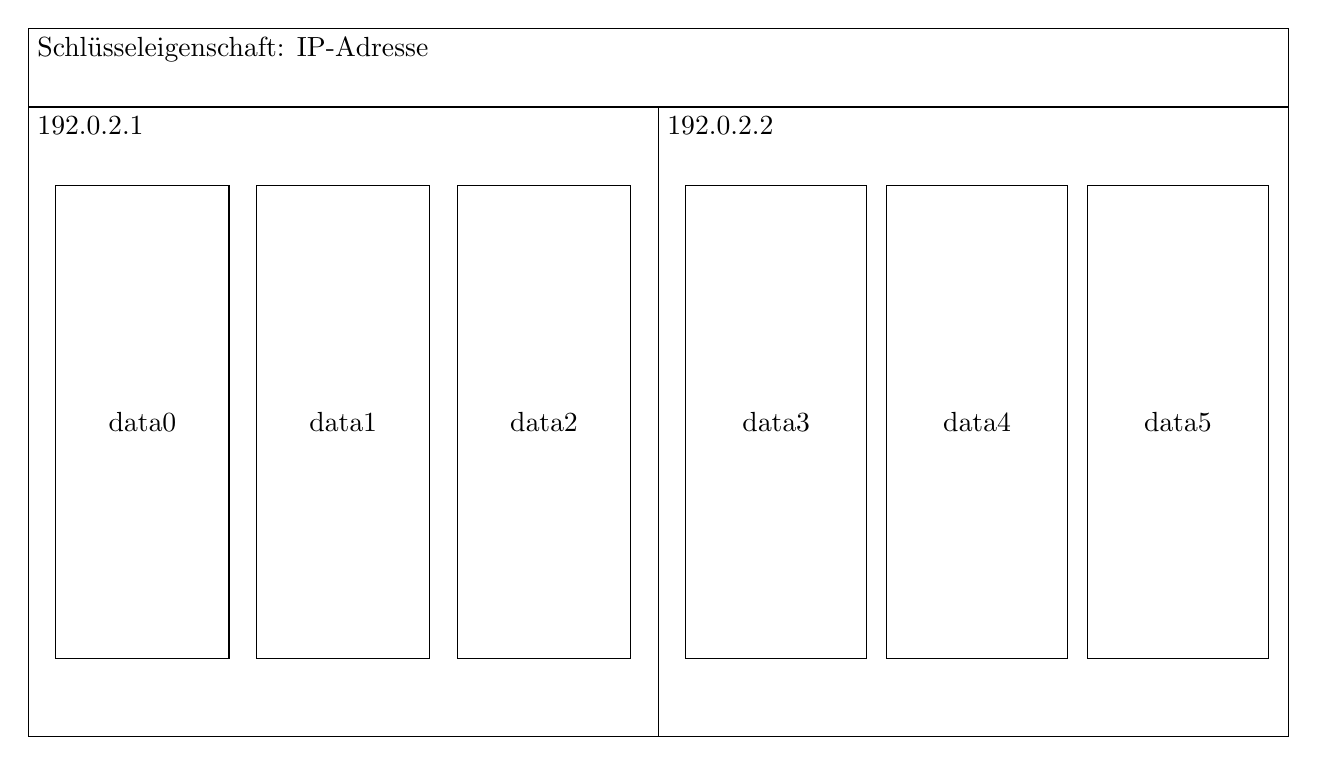
\begin{tikzpicture}
\node (rect) [rectangle, draw, minimum width=160mm, minimum height=90mm, anchor= north west] at (0,0) {};
\node [below right] at (rect.north west) {Schlüsseleigenschaft: IP-Adresse};

\node (rectA) [rectangle, draw, minimum width=80mm, minimum height=80mm, anchor= north west] at (0,-1) {};
\node [below right] at (rectA.north west) {192.0.2.1};

\node (rectA0) [rectangle, draw, minimum width=22mm, minimum height=60mm, anchor= north west] at (0.35,-2) {};
\node [] at (rectA0.center) {data0};
\node (rectA1) [rectangle, draw, minimum width=22mm, minimum height=60mm, anchor= north west] at (2.9,-2) {};
\node [] at (rectA1.center) {data1};
\node (rectA2) [rectangle, draw, minimum width=22mm, minimum height=60mm, anchor= north west] at (5.45,-2) {};
\node [] at (rectA2.center) {data2};

\node (rectB) [rectangle, draw, minimum width=80mm, minimum height=80mm, anchor= north west] at (8,-1) {};
\node [below right] at (rectB.north west) {192.0.2.2};

\node (rectB0) [rectangle, draw, minimum width=23mm, minimum height=60mm, anchor= north west] at (8.35,-2) {};
\node [] at (rectB0.center) {data3};
\node (rectB1) [rectangle, draw, minimum width=23mm, minimum height=60mm, anchor= north west] at (10.9,-2) {};
\node [] at (rectB1.center) {data4};
\node (rectB2) [rectangle, draw, minimum width=23mm, minimum height=60mm, anchor= north west] at (13.45,-2) {};
\node [] at (rectB2.center) {data5};
\end{tikzpicture}
\caption{Schematische Darstellung der Visualisierungsmöglichkeiten der Baumstruktur}
\label{fig:schem}
\end{figure}

\textit{geografische Karte}: Die Verwendung der Darstellung der Dateien als Standpunkte auf einer Karte basiert auf den Eigenschaften Lat (Latitude - Breitengrad) und Lon (Longitude - Längengrad) der Model-Klasse.
Für die Bestimmung eines Standpunktes anhand der IP-Adresse wird die API von \url{http://ip-api.com} verwendet.
Von der API werden die Längen- und Breitengrade, sowie die Informationen zu Land, Region, Stadt und des Internetanbieters abgefragt.

\textit{Zeitstrahl}: Die Darstellung als Zeitstrahl zeigt, wie viele Dateien zu einen Zeitpunkt hochgeladen wurden.
Die X-Achse repräsentiert die Zeit und die Y-Achse die Anzahl der Dateien.

In Abbildung~\ref{fig:VisualPageAll} ist eine beispielhafte \textit{FileEntryVisual} HTML-Seite zu sehen.
Die HTML-Seite bildet im rechten Teil des Fensters eine Baumkarte ab.
%Die HTML-Seite wird eine Baumkarte dargestellt im rechten Teil des Fensters dargestellt.
Die repräsentierten Daten beziehen sich auf die Beispieldaten im Szenario des Kapitel~\ref{AliceBob} und werden dort näher beschrieben.
Im linken Bereich des Fensters ist der Navigationsbereich zu erkennen.
Es wird das ausgewählte \textit{Set A} angezeigt, welches die ungeschützten Daten repräsentiert.
Für das Wechseln zwischen den beiden Datenmengen \textit{Set A} und \textit{Set B} sind zwei Schaltflächen mit den Beschreibungen A und B zu erkennen.
Unter den beiden Schaltflächen sind zwei Auswahlmenüs platziert. 
Das Obere zur Auswahl der Visualisierung, das Untere zur Auswahl der Schlüsseleigenschaft, welche zum Erstellen der Baumkarte benötigt wird.
Darunter sind die verschiedenen Eigenschaften für eine ausgewählte Datei aufgelistet.
Die ausgewählte Datei in der Abbildung ist dataAlice1, welche in der Visualisierung im rechten Teil des Fensters als grüne Box zu erkennen ist.
Durch das Anklicken einer Box werden die Eigenschaften dieser Datei angezeigt.
\begin{figure}[H]
\includegraphics[width=0.7\textwidth]{../pic/VisualPageAll.png}
\captionof{figure}{FileEntryVisual HTML-Seite mit Beispieldaten aus Kapitel~\ref{Kap:Szenarios}}
\label{fig:VisualPageAll}
\end{figure}

\chapter{Szenarien} \label{Kap:Szenarios}

Um die Visualisierungen erzeugen zu können werden Daten benötigt, die verschiedenen Benutzern gehören.
Diese Daten sollen wie bereits ausgeführt als geschützte Daten und ungeschützte Daten vorhanden sein. 
Dafür werden im folgenden zwei Szenarien definiert, anhand welcher die Visualisierungen beispielhaft dargestellt werden. 
Diese Beispiele basieren nicht auf Echtdaten.
Die Daten wurden so gewählt, dass der Effekt durch die Visualisierung präsentiert werden kann.
Die Verkehrs- und Metadaten werden für jeden Benutzer so gewählt, dass diese sich unterscheiden. 
Für die genauen Daten werden Standartwerte und Beispieldaten aus anderen Quellen verwendet. 
Für die benutzten IP-Adressen wurden die nach \cite{RFC5737} gewählten IP-Adressen für Dokumentationszwecke gewählt.
Die Werte für die Header \textit{Accept} und \textit{Accept-Encoding} entsprechen den Beispielen aus \cite[sec. 5.3.2]{RFC7231} und \cite[sec. 5.3.4]{RFC7231}.
Der Header \textit{User-Agent} für die Benutzer wurden aus \cite{MDN} übernommen.

    \section{Beispiel: Alice und Bob} \label{AliceBob}
Um die Visualisierungen an einem Beispiel zu erläutern wird ein Szenario definiert, welches die Benutzung des Dokumentenspeichers und die verwendeten Daten beschreibt.
Dazu werden zwei Benutzer Alice und Bob definiert, welche sich beide in Hamburg befinden und sich in den Verkehrs- und Metadaten unterscheiden, sodass sie anhand dieser klar unterschieden werden können.
Alice und Bob laden jeweils drei Dateien mit und ohne die Verwendung einer Methode zum Anonymisieren ihrer Daten hoch.
Alice Dateien sind dataAlice1, dataAlice2 und dataAlice3 und Bobs Dateien sind dataBob1, dataBob2 und dataBob3 und haben alle unterschiedliche Dateigrößen.
Die Verkehrs- und Metadaten für diese Dateien sind so gewählt, dass sich die Verkehrsdaten von Alice und Bob im \textit{User-Agent} Headerfeld unterscheiden.
Es wird angenommen, dass die Dateien von Alice einzeln in einem Abstand von mindestens zehn Minuten hochgeladen werden.
Die Dateien von Bob werden alle zusammen in einem Dateiupload hochgeladen.
Für die Verwendung einer Methode zum Anonymisieren ihrer Daten werden zwei Fälle betrachtet:
\begin{enumerate}
\item Die Verwendung eines Proxys, welcher von Alice und Bob verwendet wird.
\item Die Verwendung des Tor-Netzwerks von Alice und Bob.
\end{enumerate}
Für den Proxy nehmen wir an, dass die End-to-End Header \cite[sec. 13.5.1]{HTTP} unverändert übermittelt werden.
Bei der Verwendung des Tor-Netzwerks nehmen wir an, dass Alice und Bob den Tor-Browser\footnote{\url{https://www.torproject.org/projects/torbrowser.html.en}} verwenden und die Standarteinstellungen des Browsers nicht verändert haben.
Das Tor-Netzwerk ist einfach beschrieben ein Netzwerk aus Rechnern, welches dazu da ist den Datenverkehr der Benutzer zu anonymisieren.
Auf die genaue Funktionsweise des Tor-Netzwerks und des Tor-Browsers wird hier nicht eingegangen, sondern auf \cite{Tor} verwiesen.

Die zu visualisierenden Daten bestehen demnach aus drei Datenmengen:
\begin{itemize}
\item der ungeschützten Datenmenge
\item der durch einen Proxy geschützten Datenmenge
\item und der durch die Verwendung der Tor-Browsers geschützten Datenmenge.
\end{itemize}
Die Visualisierungen dieser drei Datenmengen werden in den folgenden Abschnitten vorgestellt und ausgewertet.

Für die Benutzer nehmen wir folgende Verkehrs- und Metadaten an: 
\paragraph{Alice}
\begin{itemize}
  \item IP: 
  \begin{itemize}
  \item IP-Adresse: 192.0.2.1
  \item Lat: 53.5770988464355 Lon: 10.0190000534058
  \item Land: Deutschland Region: Hamburg Stadt: Hamburg
  \end{itemize}
  \item Headerfingerprint: \textit{764529ca99fefafd6f805bca7f2e5194} aus :
  \begin{itemize}
  \item \textit{Accept}: text/*, text/plain, text/plain;format=flowed, */*
  \item \textit{Accept-Encoding}: compress, gzip
  \item \textit{User-Agent}: Mozilla/5.0 (Macintosh; Intel Mac OS X x.y; rv:42.0) Gecko/20100101 Firefox/42.0
  \end{itemize}
\end{itemize}

\paragraph{Bob}
\begin{itemize}
  \item IP: 
  \begin{itemize}
  \item IP-Adresse: 192.0.2.2
  \item Lat: 53.5830001831055 Lon: 9.98130035400391
  \item Land: Deutschland Region: Hamburg Stadt: Hamburg
  \end{itemize}
  \item Headerfingerprint: \textit{f0ed0280bb701436185829473d55a185} aus:
  \begin{itemize}
  \item \textit{Accept}: text/*, text/plain, text/plain;format=flowed, */*
  \item \textit{Accept-Encoding}: compress, gzip
  \item \textit{User-Agent}: Mozilla/5.0 (Windows NT 6.1; Win64; x64; rv:47.0) Gecko/20100101 Firefox/47.0
  \end{itemize}
\end{itemize}

\subsection{IP-Adressen bezogene Visualisierung} \label{ipVis}

In den weiteren Abbildungen dieses Kapitels werden immer die Beispieldaten von Alice und Bob mit dem Visualisierungstool des Dokumentenspeichers dargestellt.

Die Abbildung~\ref{fig:ungIpTM} zeigt die Visualisierung der Baumkarte für die Datenmenge der ungeschützten Dateien nach dem schematischem Beispiel aus Abbildung~\ref{fig:schem}. 
In Abbildung~\ref{fig:ungIpTM} ist eine blaue Box als Wurzelknoten zu erkennen, welche den Titel: \glqq \textit{Key: ipAddress}\grqq ~trägt und damit die gewählte Schlüsseleigenschaft benennt.
In diese Box sind zwei orange Boxen eingebettet.
Beide Boxen tragen einen Titel, der obere \glqq \textit{Key: 192.0.2.1}\grqq, die IP-Adresse von Alice, und der untere \glqq \textit{Key: 192.0.2.2}\grqq, die IP-Adresse von Bob.
Die obere Box (mit Alices IP-Adresse betitelt) sind drei weitere grüne Boxen eingebettet, welche für die Dateien dataAlice1, dataAlice2 und dataAlice3 stehen.
In der unteren Box (mit Bobs IP-Adresse betitelt) sind drei rote Boxen eingebettet, welche die Dateien dataBob1, dataBob2 und dataBob3 darstellen.
Die Farbe der einzelnen Boxen ist abhängig von dem jeweiligen Elternknoten in der Baumstruktur, sodass Kindknoten eines Knoten immer gleich eingefärbt sind.
Somit wird die Zusammengehörigkeit von Dateien anhand der farblichen Markierung sofort sichtbar.
Die blaue Box stellt immer den Wurzelknoten dar, die orangenen dessen Kindknoten, welche die Einträge für die gewählte Schlüsseleigenschaft der gesammelten Verkehrs- und Metadaten sind.
Hier in diesem Beispiel die IP-Adressen von Alice und Bob.

\begin{figure}[H]
\includegraphics[width=0.7\textwidth]{../pic/vec/IP-Proxy-SetA-tree3.png}
\captionof{figure}{Baumkarte der IP-Adressen der ungeschützten Beispieldaten von Alice und Bob}
\label{fig:ungIpTM}
\end{figure}

In Abbildung~\ref{fig:ungIpM} ist eine Karte von Hamburg Zentrum zu erkennen.
Auf dieser Karte sind 2 Standpunkte markiert.
Ein Punkt liegt bei Lat: 53.5770988464355 Lon: 10.0190000534058, welcher aus der IP-Adresse von Alice ermittelt wurde und dem definierten Standpunkt von Alice entspricht.
Der zweite Punkt liegt bei Lat: 53.5830001831055 Lon: 9.98130035400391, welcher aus der IP-Adresse von Bob ermittelt wurde und dem im Szenario definierten Standpunkt von Bob entspricht.
Beim Überfliegen eines Punktes mit der Maus wird im Szenario für jeden Punkt die zugehörige IP-Adresse als Tooltip\footnote{siehe \url{https://en.wikipedia.org/wiki/Tooltip}} angezeigt und die Anzahl von Dateien, welche von dieser IP-Adresse hochgeladen wurden.

\begin{figure}[H]
\includegraphics[width=0.5\textwidth , height=0.4\textheight]{../pic/IP-Proxy-SetA.PNG}
\captionof{figure}{Standorte ermittelt aus den ungeschützten Beispieldaten von Alice und Bob}
\label{fig:ungIpM}
\end{figure}

Die Darstellung der Daten spiegelt somit die definierten Beispieldaten korrekt wieder und erlaubt es die jeweiligen Daten den richtigen Benutzern zuzuordnen. 
Der Servicebetreiber kennt somit die Position von Alice und Bob und kann die von ihnen hochgeladenen Dateien durch die IP-Adresse identifizieren.

Für die Verwendung von datenschutzfreundlichen Methoden zum Anonymisieren von Daten ergeben sich de folgenden Abbildungen.

Beim Betrachten des ersten Falls, der Verwendung eines Proxys, ergeben sich die Visualisierungen wie in Abbildung~\ref{fig:PIpTM} und Abbildung~\ref{fig:PIpM}.
In Abbildung~\ref{fig:PIpTM} ist nur eine orangene Box für die IP-Adresse des Proxys dargestellt.
Alle sechs definierten Dateien, die Dateien von Alice dataAlice1, dataAlice2 und dataAlice3 und die Dateien von Bob dataBob1, dataBob2 und dataBob3, sind dieser IP-Adresse zugeordnet und als grüne Boxen unter der IP-Adresse des Proxys angeordnet.
In Abbildung~\ref{fig:PIpM} ist ein Standpunkt in Berlin markiert.
Der Standpunkt liegt bei Lat: 52.5167 Lon: 13.4 und ist durch die IP-Adresse des Proxys ermittelt worden. 

\begin{figure}[H]
\includegraphics[width=0.7\textwidth]{../pic/IP-Proxy-SetB-tree3.PNG}
\captionof{figure}{Baumkarte der IP-Adresse der Beispieldaten von Alice und Bob bei der Verwendung eines Proxys}
\label{fig:PIpTM}
\end{figure}

\begin{figure}[H]
\includegraphics[width=0.5\textwidth , height=0.2\textheight]{../pic/IP-Proxy-SetB.PNG}
\captionof{figure}{Standorte von Alice und Bob bei der Verwendung eines Proxys}
\label{fig:PIpM}
\end{figure}

Beim Vergleich der Abbildungen~\ref{fig:ungIpTM} und \ref{fig:PIpTM} sowie \ref{fig:ungIpM} und \ref{fig:PIpM} ist klar zu erkennen, dass durch die Verwendung eines Proxys, der Servicebetreiber die einzelnen Dateien nicht mehr anhand der IP-Adresse deren tatsächlichen Besitzern zuordnen kann.
Die Zuordnung der Dateien zu einer einzelnen IP-Adresse lässt dem Servicebetreiber bei der alleinigen Betrachtung der IP-Adresse nur darauf schließen, dass alle Dateien von demselben Benutzer stammen.
Die Dateien von Alice und Bob sind somit durch die Verwendung des Proxys durch eine Anonymitätsmenge geschützt, sodass die Dateien in der durch die IP-Adresse erzeugte Gruppierung anonym werden.
Da die Beispieldaten zwei Benutzer definieren und der Servicebetreiber anhand des verwendeten Proxys nur auf einen Benutzer schließen kann, ist der Effekt durch die Verwendung des Proxys klar anschaulich geworden. 

Abbildung~\ref{fig:TIpTM} und \ref{fig:TIpM} zeigen die Visualisierungen für die Verwendung des Tor-Netzwerks als Methode zum Anonymisieren der Daten.
In der Abbilung~\ref{fig:TIpTM} sind vier verschiedene orange Boxen für vier verschiedene IP-Adressen abgebildet.

Die Zuordnung der Dateien zu den IP-Adressen entspricht:
\begin{description}[style=nextline]
%\centering
\item[203.0.113.1] Datei: dataAlice1, Farbe: grün
\item[203.113.5] Datei: dataAlice2, Farbe: lila
\item[203.0.113.13] Datei: dataAlice3, Farbe: braun
\item[203.0.113.2] Farbe: rot
\begin{enumerate}
\item dataBob1
\item dataBob2
\item dataBob3
\end{enumerate}
\end{description}

Für jede dieser IP-Adressen ist in der Karte in Abbildung~\ref{fig:TIpM} ein Standort abgebildet, welche über Deutschland verteilt sind. 
\begin{description}
\item[1] Hermsdorf (Thüringen) - Lat: 50.8919 Lon: 11.8682
\item[2] Karlsruhe (Innenstadt-Ost) - Lat: 49.0096 Lon: 8.41217
\item[3] Frankfurt am Main - Lat: 50.1109 Lon: 8.68213
\item[4] Berlin (Charlottenburg-Wilmersdorf) - Lat: 52.5239 Lon: 13.3214
\end{description}

\begin{figure}[H]
\includegraphics[width=0.7\textwidth]{../pic/IP-Tor-SetB-tree4.png}
\captionof{figure}{Baumkarte der IP-Adresse der Beispieldaten von Alice und Bob bei der Verwendung des Tor-Netzwerks}
\label{fig:TIpTM}
\end{figure}

\begin{figure}[H]
\includegraphics[width=0.4\textwidth]{../pic/IP-Tor-SetB-Map.png}
\captionof{figure}{Standorte der Dateien von Alice und Bob bei der Verwendung des Tor-Netzwerks}
\label{fig:TIpM}
\end{figure}

Vergleicht man wiederum Abbildung~\ref{fig:ungIpTM} mit \ref{fig:TIpTM} und \ref{fig:ungIpM} mit \ref{fig:TIpM} fallen deutliche Unterschiede in den Visualisierungen auf. 
Während, wie bereits (oben) ausgeführt, in Abbildung~\ref{fig:ungIpTM} die Beispieldaten korrekt gruppiert visuell dargestellt werden,
lässt die Darstellung aus Abbildung~\ref{fig:TIpTM} und Abbildung~\ref{fig:TIpM} dies nicht mehr zu.
Die Dateien von Bob können zwar zusammen gruppiert werden, jedoch sind die Dateien von Alice auf drei verschiedene IP-Adressen verteilt.
Die Gruppierung der Dateien von Bob ist zwar korrekt jedoch entspricht die IP-Adresse und somit auch der Standort, der daraus abgeleitet ist, nicht mehr dem definierten Standort was darauf zurückzuführen ist, dass die Dateien alle zusammen hochgeladen wurden.
Ein Servicebetreiber muss so anhand der IP-Adresse annehmen, dass die Dateien von vier verschiedenen Benutzern stammen.
Dies widerspricht klar den definierten Daten und zeigt die Anonymisierung der Daten durch die Verwendung des Tor-Netzwerks.

Die Betrachtung beider Fälle von Anonymisierung (Verwendung eines Proxys oder des Tor-Netzwerks) ergibt, das beide Schutzmethoden im Hinblick auf die IP-Adresse einen derart ausreichenden Effekt gehabt haben, dass eine korrekte Zuordnung von Datei und Benutzer bezüglich der IP-Adresse nicht mehr möglich waren.

\subsection{Headerfingerprint bezogene Visualisierung}
Nach der Auswertung der Informationen, welche aus der IP-Adressbezogenen Visualisierung abgeleitet werden können, kann ein Servicebetreiber weitere der gesammelten Eigenschaften untersuchen um festzustellen, ob andere Eigenschaften die gleichen Schlussfolgerungen erlauben wie die IP-Adresse und diese somit erhärten oder ob andere Eigenschaften zu anderen Schlussfolgerungen führen.

Um die Veränderungen bezüglich des Headerfngerprints visualisieren zu können, muss in der \textit{FileEntryVisual} HTML-Seite im Navigationsbereich die Schlüsseleigenschaft auf den \textit{Headerfingerprint} umgestellt werden.

Für die ungeschützten Beispieldaten von Alice und Bob erhalten wir die Visualisierung als Baumkarte, wie sie in  Abbildung~\ref{fig:ungHTM} gezeigt wird.
Zu erkennen sind zwei orange Boxen für die beiden verschiedenen Headerfingerprints.
Der oberen orangen Box mit dem Headerfingerprint \textit{764529ca99fefafd6f805bca7f2e5194} sind drei Dateien dataAlice1, dataAlice2 und dataAlice3 zugeordnet, welche alle farblich grün markiert sind.
Der unteren orangen Box mit dem Headerfingerprint  \textit{f0ed0280bb701436185829473d55a185} sind die drei Dateien dataBob1, dataBob2 und dataBob3 zugeordnet, welche farblich rot markiert sind.

\begin{figure}[H]
%\includegraphics[width=0.7\textwidth]{../pic/IP-Tor-SetB.png}
\includegraphics[width=0.7\textwidth]{../pic/Header-Proxy-SetA2.png}
\captionof{figure}{Baumkarte der Beispieldaten von Alice und Bob bei Betrachtung der Schlüsseleigenschaft: Headerfingerprint}
\label{fig:ungHTM}
\end{figure}

Wie in Abbildung~\ref{fig:ungIpTM} stellt Abbildung~\ref{fig:ungHTM} die Zusammengehörigkeit der Dateien dataAlice1, dataAlice2 und dataAlice3 sowie den Dateien dataBob1, dataBob2 und dataBob3 richtig dar.

Die Verwendung des Proxys hat keinen Effekt bezüglich der Visualisierung des Headerfingerprints und entspricht somit der Abbildung~\ref{fig:ungHTM}.
Dies ist darauf zurückzuführen, dass die Verwendung des Proxys die Header-Felder \textit{User-Agent}, \textit{Accept} und \textit{Accept-Encoding} nicht verändert und die eigentlichen Werte von Alice und Bob weitergegeben werden.

Bei Betrachtung des zweiten Falls, der Verwendung des Tor-Netzwerkes, entspricht die Visualisierung der Abbildung~\ref{fig:THTM}.
Zu erkennen ist, dass ähnlich der Abbildung~\ref{fig:PIpTM} alle Dateien unter einem Headerfingerprint \textit{274e7dc5014d882a1cf8756d0600a52a} angeordnet sind (die Datei dataBob3 ist mit einem X dargestellt, da nicht genung Platz ist, um den Dateinamen anzuzeigen).
Dies ist darauf zurückzuführen, dass durch die Verwendung des Tor-Browsers Alice und Bob standardisierte Werte für die Header-Felder \textit{User-Agent}, \textit{Accept} und \textit{Accept-Encoding} verwenden.
Die standartisierten Felder erzeugen einen identischen Headerfingerprint für Alice und Bob.

\begin{figure}[H]
\includegraphics[width=0.7\textwidth]{../pic/Header-Tor-SetB2.png}
\captionof{figure}{Baumkarte des Headerfingerabdrcuks der Beispieldaten von Alice und Bob geschützt druch die Verwendung des Tor-Netzwerks}
\label{fig:THTM}
\end{figure}

Die Verwendung des Tor-Browsers hat somit zur Folge, dass die Dateien und Alice und Bob alle unter einem einzelnen Headefingerprint gruppiert werden. 
Für den Servicebetreiber bedeutet dies, dass anhand des Headerfingerprints anzunehmen ist, dass die Dateien alle von einem einzelnen Benutzer stammen. 
Der Effekt der Verwendung des Tor-Netzwerks und -Browsers ist so sichtbar, da die Informationen, die ein Servicebetreiber ableiten kann, sich von denen der ungeschützten Daten unterscheiden.

Da die Verwendung des Proxys keinen Effekt auf die für den Headerfingerprint ausschlaggebenden Header hatte, ist der Headerfingerprint der Benutzer trotz Benutzung des Proxys gleich geblieben. 
Die Verwendung des Tor-Netzwerks hat hingegen dazu geführt, dass die Headerfingerprints von Alice und Bob, aus dem ungeschützten Beispiel, beide durch einen standardisierten Headerfingerprint ersetzt wurden und somit die korrekte Zuordnung der Dateien zu den jeweiligen Benutzern nicht mehr möglich war.

Die Verwendung des Tor-Netzwerks hat somit eine Anonymitätsmenge für die Eigenschaft des Headerfingerprints erzeugt, in welcher die Dateien anonym sind und den Benutzern Alice und Bob nicht zugeordnet werden können.

\subsection{Vergleich der Schutzmethoden}

Die Visualisierungen haben eindeutig und anschaulich gezeigt, dass die Verwendung eines Proxys im Hinblick auf die IP-Adresse (Abbildung~\ref{fig:PIpTM}) nicht aber im Hinblick auf den Headerfingerprint (Abbildung~\ref{fig:ungHTM}) einen anonymisierenden Schutz bewirkt.
So wird durch die Verwendung eines Proxys die eigentliche IP-Adresse des Benutzers durch die des Proxys maskiert, der Headerfingerprint des Benutzer jedoch nicht verändert.
Sollten mehrere Benutzer den gleichen Proxy verwenden (wie im Beispiel von Alice und Bob) können die Dateien dieser Nutzer anhand der IP-Adresse nicht mehr korrekt zugeordnet werden. 
Sollte jedoch ein Benutzer einen Proxy alleine benutzen, so kann der Proxy lediglich die IP-Adresse des Benutzer maskieren, erlaubt jedoch immer noch die Zuordnung der Dateien über z.~B. den Headerfingerprint.
Da der Headerfingerprint nicht verändert wird, kann ein Benutzer trotz der Verwendung eines Proxys über seinen Headerfingerprint identifiziert werden, falls dieser einzigartig genug sein sollte.
Nach dem Beispiel der Visualisierungen für die Verwendung des Proxys
hat ein Servicebetreiber verschiedene sich widersprechende Auslegungsmöglichkeiten für die visualisierten Daten.
Aus der IP-Adresse kann ein Servicebetreiber nur auf einen Benutzer schließen, der sechs Dateien hochgeladen hat.
Aus dem Headerfingerprint kann jedoch auf zwei verschiedene Benutzer geschlossen werden. 
Ein Servicebetreiber muss anhand dieser Informationen nun abwägen, welche der Schlussfolgerungen wahrscheinlicher ist. 
Ein Servicebetreiber kann annehmen, dass alle Dateien von einem Benutzer stammen und z. B. durch die Verwendung eines anderen Browser oder durch ein Update des verwendeten Browsers sich der Headerfingeprint des Benutzers geändert hat.
Oder es wird angenommen, dass es zwei Benutzer gibt, welche einen verschiedenen Headerfingerprint besitzen und z. B. durch die Verwendung eines Proxys, wie in dem Beispiel angenommen, ihre IP-Adresse maskieren.
Sollte ein Servicebetreiber die Gänze der gesammelten Eigenschaften der Dateien von Bob betrachten wäre so auffällig, dass die drei Dateien alle identische Verkehrsdaten haben.
Ob die restlichen Dateien ebenfalls zu diesem Benutzer oder anderen Benutzern gehören ist anhand der betrachteten Informationen nicht eindeutig festzustellen.
Die Verwendung des Tor-Netzwerks dagegen kann, wie in Abbildung~\ref{fig:TIpTM} und Abbildung~\ref{fig:THTM} gezeigt, Schutz vor der Identifizierung durch die IP-Adresse und den Headerfingerprint bieten.
Dabei ist zu beachten, dass die während durch die Visualisierung aus Abbildung~\ref{fig:TIpTM} ein Servicebetreiber von vier Benutzern ausgehen muss.
Die Visualisierung in Abbildung~\ref{fig:THTM} nur auf einen Benutzer schließe lässt.
Dass Bob in diesem Beispiel die Dateien alle als ein Dateiupload hochlud, macht seine Dateien leicht eindeutig zuordbar, da das Hochladen der Dateien in einer Anfrage an den Dokumentenspeicher dieses trivialisiert.

Aus dem definierten Szenario lässt sich schließen, dass während die Verwendung eines Proxys und des Tor-Netzwerks im Hinblick auf die Anonymisierung der IP-Adresse gleich erfolgreich seien können, die Verwendung eines Proxys gegenüber dem Tor-Netzwerk jedoch einen deutlichen Nachteil hat, bezogen auf die Möglichkeit durch seinen eigenen individuellen Headerfingerprint identifiziert zu werden.
Auch dass Dateien einzeln hochgeladen werden sollten, ist anhand der Identifikation der Zusammengehörigkeit der Dateien von Bob sichtbar geworden. 

\section{Beispiel: Adam, Beth und Chris} \label{Kap:ABC}
Wie in Kapitel~\ref{AliceBob} wird ein Beispielszenario für die Vorstellung einer Visualisierungsmöglichkeit definiert.
Die zu betrachtende Visualisierung ist der Zeitstrahl.
Dafür werden drei Benutzer definiert, sowie ein Proxy, welcher als Schutzmethode verwendet wird.
Die drei Benutzer laden jeweils mehrere Dateien hoch:
\begin{itemize}
\item Adam: drei Dateien
\item Beth: drei Dateien
\item Chris: zwei Dateien
\end{itemize}
Die Dateien von Adam werden täglich um 05:30 Uhr hochgeladen.
Die Dateien von Beth werden am 26.6. um :
\begin{itemize}
\item 17:31 Uhr,
\item 18:10 Uhr und
\item 19:54 Uhr
\end{itemize}
hochgeladen.
Die Dateien von Chris werden zusammen am 28.6. um 12.21 Uhr hochgeladen.
Da die Visualisierung von IP-Adresse und Headerfingerprint bereits in Kapitel~\ref{AliceBob} behandelt wurden, werde diese Verkehrsdaten der Benutzer für dieses Beispiel vernachlässigt.
Der Proxy, welcher als Schutzmethode verwendet wird, funktioniert wie folgt.
Jede hochgeladene Datei wird im Proxy in einem Puffer gespeichert und dieser Puffer wird täglich um 00:00 Uhr einmal geleert, indem die gesammelten Dateien an den Dokumentenspeicher geschickt werden. 

\subsection{Zeitbezogene Visualisierung}
In der zeitbezogenen Visualisierung werden die Zeitstempel verwendet, wann eine Datei hochgeladen wurde, um eine Visualisierung zu erzeugen.
Diese Visualisierung zeigt wie viele Dateien zu welchem Zeitpunkt hochgeladen wurden.

In Abbildung~\ref{fig:ungTime} sind die ungeschützten Daten von Adam, Beth und Chris dargestellt.
Die Dateien von Adam sind jeweils einzeln am 26.6., 27.6. und 28.6. um 5:30 Uhr zu erkennen.
Die Dateien von Beth sind am 26.6. zwischen 17 und 20 Uhr abgebildet.
Die Dateien von Chris sind am 28.6. zu erkennen und sind in einem Zeitpunkt mit der Mächtigkeit zwei zusammengefasst, da diese Dateien zum gleichen Zeitpunkt hochgeladen wurden.

\begin{figure}[H]
\includegraphics[width=0.7\textwidth]{../pic/TimeLine-SetA2.png}
\captionof{figure}{Zeitstrahl der ungeschützten Beispieldaten von Adam, Beth und Chris}
\label{fig:ungTime}
\end{figure}

Das regelmäßige Hochladen der Dateien von Adam ist in der Abbildung zu erkennen.
Die immer gleich bleibenden Abstände zwischen den blauen Balken kann als ein Indiz dafür genommen werden, dass diese von demselben Benutzer stammen.
Dies ist auch der Fall für die Dateien von Chris, da sie in einem Upload hochgeladen wurden und somit einen identischen Zeitstempel haben.
Bei den Dateien von Beth ist eine Zuordnung nicht möglich, da die Zeitpunkte des Hochladens unregelmäßige Abstände haben.

Um diese möglichen Gruppierungen der Dateien von Adam und Chris aufzulösen,
verwenden nun alle drei Benutzer den in Kapitel~\ref{Kap:ABC} definierten Proxy.

In der Abbildungs~\ref{fig:ProxyTime} ist nun die Visualisierung der gesammelten Daten bei der Verwendung des Proxys zu sehen.
Wie nach Definition des Proxys gibt es nur drei Punkte im betrachteten Zeitraum, jeweils um 00:00 Uhr:
\begin{itemize}
\item 27.6.: 4 Dateien,
\item 28.6.: 1 Datei,
\item 29:6.: 3 Dateien.
\end{itemize}
Die Dateien vom 27.6. bestehen aus einer Datei von Adam und den drei Dateien von Beth.
Die Dateien vom 29.6. bestehen aus einer Datei von Adam und den beiden Dateien von Chris.
Die Datei vom 28.6 ist die Datei von Adam.

\begin{figure}[H]
\includegraphics[width=0.7\textwidth]{../pic/TimeLine-SetB.png}
\captionof{figure}{Zeitstrahl der durch einen Proxy geschützten Beispieldaten von Adam, Beth und Chris}
\label{fig:ProxyTime}
\end{figure}

Da für alle Dateien, die einen identischen Zeitstempel haben, angenommen werden kann, dass sie von demselben Benutzer stammen, ergibt sich bereits eine Veränderung bei der Zuordbarkeit der Daten von Adam und Chris.
Da die zeitlichen Abstände zwischen den Uploads auch gleich sind, lässt sich weiter schließen, dass alle Dateien zusammengehörig sind.
Ein Servicebetreiber kann so anhand der Visualisierung auf einen Benutzer, was dem Proxy entsprechen würde, schließen, jedoch nicht auf die Benutzer des Proxys.

Wie aus der Abbildung~\ref{fig:ungTime} abgeleitet werden konnte, gelingt die Gruppierung der Dateien von Adam und Chris, wenn diese ihre Dateien ohne die Verwendung einer Schutzmethode hochladen.
Diese Gruppierung kann bei Nutzung des Proxys, wie sie in Kapitel~\ref{Kap:ABC} festgelegt wurde, nicht mehr erfolgen.
%Während die ungeschützten Daten die Gruppierung der Dateien von Adam und Chris zulassen.
%Kann bei der Verwendung des Proxys nach Kapitel~\ref{Kap:ABC}, diese Zuordnungmöglichkeit aufgehoben werden.
Dabei sind jedoch zwei Dinge zu beachten. 
Die Benutzung des Dokumentenspeichers ist durch den Proxy erheblich verzögert, da die Dateien im Puffer des Proxys auf die Weiterleitung an den Dokumentenspeicher warten müssen.
Während der Wartezeit können die Dateien z.~B. nicht durch den Dokumentenspeicher zugänglich gemacht werden.
Genauso ist zu beachten, dass die Verwendung des Proxys zwar den Servicebetreiber des Dokumentenspeichers daran hindert die originalen Zeitstempel der Dateien zu erfassen, der Servicebetreiber des Proxys jedoch immer noch dazu in der Lage ist.

\section{Zusmamenfassung der Visualisierungen}
In Kapitel~\ref{AliceBob} wurde anhand des Beispiels von Alice und Bob die Darstellungsmethode der Baumkarte und der Darstellung von Standpunkten auf einer Karte vorgestellt.
Dabei wurde die Verwendung eines Proxys und des Tor-Netzwerks und Tor-Browsers als Schutzmethoden exemplarisch an Beispieldaten visualisiert und ausgewertet.
Beide Methoden wurden hinsichtlich der Eigenschaft der IP-Adresse und des Headerfingerprints untersucht und eine Aussage darüber getroffen, inwiefern diese sich im gegebenen Beispiel eignen, um eine der beiden Eigenschaften zu anonymisieren.

In Kapitel~\ref{Kap:ABC} wurde anhand eines Beispiels von drei Benutzern die Darstellungsmethode des Zeitstrahls vorgestellt.
Dabei wurde ein Proxy mit einem bestimmten definierten Verhalten als Schutzmethode eingesetzt.
Es wurde gezeigt, dass durch die Betrachtung von regelmäßig auftretenden Zeitstempeln oder bei identischen Zeitstempeln Gruppierungen erzeugt werden können und wie ein speziell definierter Proxy dies verhindern kann.
% Schluss
\chapter{Schluss}
\section{Zusammenfassung der Ergebnisse}

Im Rahmen dieser Arbeit wurde ein einfacher Dokumentenspeicher sowohl konzipiert als auch implementiert.
Entsprechend der Aufgabenstellung ist das Verhalten des Dokumentenspeichers so gewählt, dass die Verkehrs- und Metadaten der hochgeladenen Dateien gesammelt und anschließend visualisiert werden.
Dazu wurden verschiedene Verwendungsmöglichkeiten im Hinblick auf das Hochladen von Dateien geschaffen.
Zur Darstellung der gesammelten Daten und der angewendeten Schutzfunktion wurden verschiedene Visualisierungsmöglichkeiten implementiert.
Diese Visualisierungsmöglichkeiten werden anhand zweier Beispielszenarien vorgestellt.
Durch die Szenarien wird die Benutzung des Dokumentenspeichers mit und ohne die Verwendung von datenschutzfreundlichen Methoden zum Anonymisieren von Daten vorgestellt.
Es wurden verschiedene Methoden zum Anonymisieren von Daten betrachtet.
Die Unterschiede zwischen anonymisierten Daten und nicht anonymisierten Daten sowie den gewählten Methoden werden anhand von Abbildungen gezeigt und ausgewertet.
Die Auswertung stellt vor allem geschützte und ungeschützte Datenmengen gegenüber.
Anhand der Visualisierungen und der Auswertung kann eingeschätzt werden, welchen Effekt die Verwendung einer datenschutzfreundlichen Methode zum Anonymisieren von Daten auf die Möglichkeiten hat, wie ein Servicebetreiber aus den Verkehrs- und Metadaten Informationen über den Besitzer der gespeicherten Daten ableiten kann.

\section{Limitierungen \& Ausblick}
Der Dokumentenspeicher erfüllt seine Funktion gemessen an seinem Verwendungszweck, jedoch gibt es einige Aspekte, anhand welcher der Dokumentenspeicher verbessert werden kann.
Momentan ist der Dokumentenspeicher sehr einfach aufgebaut und hat nur eine kleine Menge an Features.
Es können Dateien hoch- und runtergeladen und die gesammelten Verkehrs- und Metadaten anhand weniger einfacher Visualisierungen dargestellt werden.

Erweiterungsmöglichkeiten ergeben sich im Bereich des Funktionalität des Dokumentenspeichers.
Es könnten Features, wie das Ersetzten von bereits hochgeladenen Dateien durch eine neue Version dieser Datei, implementiert werden.
Genauso könnten die HTML-Seiten hinsichtlich der Benutzerfreundlichkeit und ihres Aussehens verbessert werden. 
Weiter wäre es sinnvoll, die verwendeten Verfahren zum Identifizieren von Benutzern, bisher hauptsächlich IP-Adresse und HTTP Fingerabdruck, durch weitere Methoden zur Identifikation eines Benutzers zu erweitern.
Die bisherigen Verfahren können so verbessert werden, dass die recht einfach gehaltene Implementation durch eine fundiertere abgelöst wird. 
Neben der Untersuchung der Verkettbarkeit der Daten können auch Ansätze erschlossen werden, welche die Metadaten der Dateien genauer betrachten und versuchen aus den Metadaten Informationen abzuleiten, die für einen Servicebetreiber von Interesse sein könnten.
Dabei könnten z.~B. untersucht werden inwiefern die Größe einer Datei auf den Dateityp oder Dateiinhalt schließen lässt.

Die Visualisierungen selbst basieren momentan auf den einzelnen Eigenschaften, die im Dokumentenspeicher gesammelten werden. 
Diese Eigenschaften können momentan hauptsächlich durch die Baumkarte dargestellt werden.
Während dieser Ansatz hinreichend ist, um in einem einfachen dafür konstruierten Fall diese Zuordnungen zu zeigen, ist es fraglich, ob dieser Ansatz bei Echtdaten zuverlässige Ergebnisse liefert.
Neben dem Prüfen, ob die Baumkarte sich als Visualisierungsmethode eignet, sollte in weiteren Arbeiten nach anderen Visualisierungsmethoden gesucht werden, welche sich eignen, die Verkettbarkeit der Daten zu repräsentieren.
Die bisherigen Visualisierungen könnten verbessert und neue Visualisierungsmöglichkeiten geschafft werden. 
Dazu könnte die Arbeit von \textcite{Chi} verwendet werden, um eine Struktur in die Implementation der Visualisierungen einfließen zu lassen und die Implementation so zu vereinfachen.

In weiteren Arbeiten kann untersucht werden, welche Effekte die Kombination von verschiedenen Eigenschaften auf die Zuverlässigkeit der Zuordnung und die daraus resultierenden Visualisierungen hat. 
Die Ansätze aus \cite{Ecke10} können dabei weiter verfolgt werden.

Zusätzlich kann in weiteren Arbeiten ein Klient für den Dokumentenspeicher entwickelt werden, welcher dem Verwendungszweck aus Kapitel~\ref{Kap:Dokumentenspeicher} entspricht.
Der Klient sollte so eine Menge an verschiedenen Schutzfunktionen anbieten, die beim Hochladen einer Datei verwendet werden können.
Zusätzlich zum Hochladen der geschützten Datei müsste dann zum Zweck der Vergleichbarkeit auch die ungeschützte Datei hochgeladen werden.
Durch die beiden unterschiedlichen API-Endpunkte für die geschützten und ungeschützten Daten können so die für die Visualisierung verwendeten Datenmengen erzeugt werden.
Durch die Verwendung dieses Klienten würde so das Erzeugen von Beispielszenarien oder das Sammeln von Echtdaten vereinfacht werden.

\printbibliography
\end{document}
